\section{Results and discussion}
\label{sec:results}

\subsection{Regulation of the saddle under utility and feed shocks}
\label{subsec:res_shocks}
The three controllers of Section~\ref{sec:design} start at the saddle and face either a step of $+10$~K in the coolant supply temperature or a step of $+5$~K in the feed temperature, applied at $t=\tShock$~min and held for the rest of the $\horizonShock$~min horizon. Table~\ref{tab:saddle_shocks} lists the integral absolute error (IAE), the peak deviation, the total variation (TV) of the valve, the largest coolant flow and the peak-to-peak amplitude of $T$ over the last 20~min, which separates a settled response from a sustained oscillation. Figure~\ref{fig:shocks} shows the trajectories.

\begin{table*}[t]
\centering
\footnotesize
\caption{Regulation at the open-loop unstable saddle ($T_{sp}=345$ K) after shocks at $t=2$ min; metrics over $t\ge 2$ min.}
\label{tab:saddle_shocks}
\resizebox{\ifdim\width>\textwidth\textwidth\else\width\fi}{!}{%
\begin{tabular}{lcccccc}
\toprule
Shock & Architecture & IAE (K min) & Peak $|e|$ (K) & TV (L/min) & $\max q_j$ (L/min) & $T$ p-p, last 20 min (K) \\
\midrule
$\Delta T_{jf}=+10$ K & SISO SIMC & 497.11 & 19.33 & 1561.7 & 177.3 & 30.46 \\
$\Delta T_{jf}=+10$ K & Cascade & 23.28 & 1.83 & 152.9 & 97.7 & 0.36 \\
$\Delta T_{jf}=+10$ K & Cascade + FF & 12.89 & 1.01 & 96.4 & 91.6 & 0.21 \\
$\Delta T_f=+5$ K & SISO SIMC & 230.03 & 19.24 & 740.8 & 167.6 & 8.34 \\
$\Delta T_f=+5$ K & Cascade & 132.07 & 24.82 & 584.4 & 190.0 & 0.84 \\
$\Delta T_f=+5$ K & Cascade + FF & 132.07 & 24.82 & 584.4 & 190.0 & 0.84 \\
\bottomrule
\end{tabular}%
}
\end{table*}


\begin{figure*}[t]
\centering
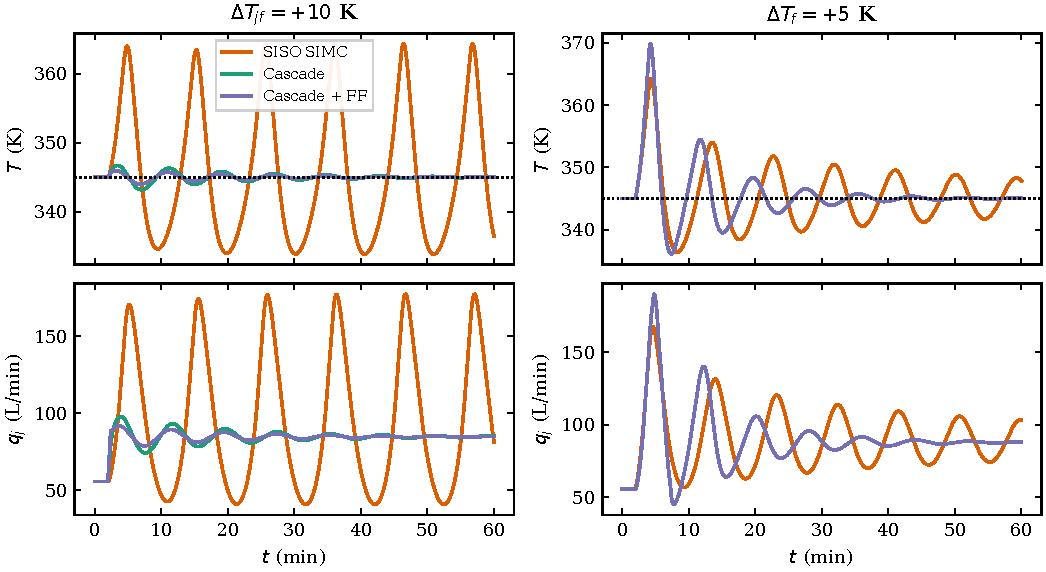
\includegraphics[width=\textwidth]{figures/fig3_saddle_shocks.pdf}
\caption{Reactor temperature (top) and coolant flow (bottom) at the saddle after a $+10$~K coolant supply shock (left) and a $+5$~K feed temperature shock (right) at $t=\tShock$~min. Dotted line: setpoint $\TSad$~K. In the right column the two cascade curves coincide because the feedforward does not measure $T_f$.}
\label{fig:shocks}
\end{figure*}

\paragraph{Coolant supply shock.} The single loop does not return to the setpoint. After the shock it enters a sustained oscillation with a peak deviation of $\peakTjfSiso$~K and a peak-to-peak amplitude of $\ptpTjfSiso$~K at the end of the run, and the valve travels $\tvTjfSiso$~L/min. The oscillation is not a slow transient. At the post-shock equilibrium ($T_{jf}=310$~K, $q_j=\qjShockTjf$~L/min) the jacket is closer to the supply temperature, the actuator gain drops to $b_3=\bThreeShockTjf$~K/L, and the linearized single loop has spectral abscissa $+\absShockTjfSiso$~min$^{-1}$: the shock moved the reactor to a point that the SISO gains no longer stabilize, and the bounded oscillation is the limit cycle of the nonlinear loop around an unstable closed-loop equilibrium. The same gains in the cascade give $\absShockTjfCascade$~min$^{-1}$ at that point. The cascade keeps the reactor within $\peakTjfCascade$~K of the setpoint and reduces the IAE by $\iaeRedTjf\%$ with less than a tenth of the valve travel. Here the classical argument for cascade control \cite{shinskey1996process,seborg2010process,astrom2006pid}, that the slave loop removes utility disturbances before they reach the reactor, holds in its strongest form: the disturbance enters the jacket balance, which is exactly the channel the slave controls. Feedforward from $T_{jf}$ through Eq.~\eqref{eq:ff} cuts the IAE by a further $\iaeRedFF\%$ and the peak deviation to $\peakTjfCascadeff$~K, because the slave bias jumps to the new equilibrium flow at the instant of the shock.

\paragraph{Feed temperature shock.} The feed shock enters the reactor energy balance directly, upstream of nothing the slave can measure. Both architectures now see a large transient: the peak deviation is $\peakTfSiso$~K for the single loop and $\peakTfCascade$~K for the cascade. The cascade still settles (peak-to-peak $\ptpTfCascade$~K over the last 20~min, linear spectral abscissa $\absShockTfCascade$~min$^{-1}$ at the post-shock equilibrium) and reduces the IAE by $\iaeRedTf\%$, whereas the single loop is still oscillating with $\ptpTfSiso$~K peak to peak after $\horizonShock$~min: its post-shock equilibrium is stable but barely ($\absShockTfSiso$~min$^{-1}$). The larger cascade peak follows from its master design: $\tau_{c1}=\theta_1$ is the default SIMC choice, not a tightened one, and the master integral time is short compared with the reactor response. As expected, the feedforward of Eq.~\eqref{eq:ff} does nothing here, and the two cascade rows coincide.

Taken together, the shocks show that at an unstable operating point the value of the cascade is not only faster disturbance rejection. The slave loop changes the plant seen by the master from unstable to stable (Section~\ref{subsec:cascade_design}), so the master can be tuned with the default SIMC rule and still keeps a stability margin when the operating point moves; the single loop, whose admissible $\tau_c$ interval is narrow (Table~\ref{tab:simc_sweep}), loses it after a moderate utility disturbance.

\subsection{Continuous fouling}
\label{subsec:res_fouling}
Table~\ref{tab:fouling} and Fig.~\ref{fig:fouling} report the fouling runs. The two operating points behave in qualitatively different ways.

\begin{table*}[t]
\centering
\footnotesize
\caption{Continuous fouling $d(UA)/dt=-\kappa_{\mathrm{foul}} r_A (UA-UA_{\min})$ with $\kappa_{\mathrm{foul}}=0.1$ L/mol and $UA_{\min}=0.30\,UA_0$. $t_{\mathrm{pred}}$: quasi-steady prediction (Eq.~\eqref{eq:t_pred}); $t_{\mathrm{sat}}$: first $q_j=u_{\max}$; $t_{\mathrm{runaway}}$: first $T-T_{sp}>5$ K.}
\label{tab:fouling}
\resizebox{\ifdim\width>\textwidth\textwidth\else\width\fi}{!}{%
\begin{tabular}{lcccccc}
\toprule
Point & Architecture & $t_{\mathrm{pred}}$ (min) & $t_{\mathrm{sat}}$ (min) & $UA(t_{\mathrm{sat}})/UA_0$ (\%) & $t_{\mathrm{runaway}}$ (min) & $T(80$ min) (K) \\
\midrule
Nominal & SISO SIMC & 8.92 & 10.02 & 57.0 & 13.18 & 416.40 \\
Nominal & Cascade & 8.92 & 9.26 & 59.0 & 13.18 & 416.40 \\
Saddle & SISO SIMC & 46.36 & 32.32 & 44.8 & 28.06 & 387.87 \\
Saddle & Cascade & 46.36 & 33.06 & 43.3 & 4.06 & 387.88 \\
\bottomrule
\end{tabular}%
}
\end{table*}


\begin{figure*}[t]
\centering
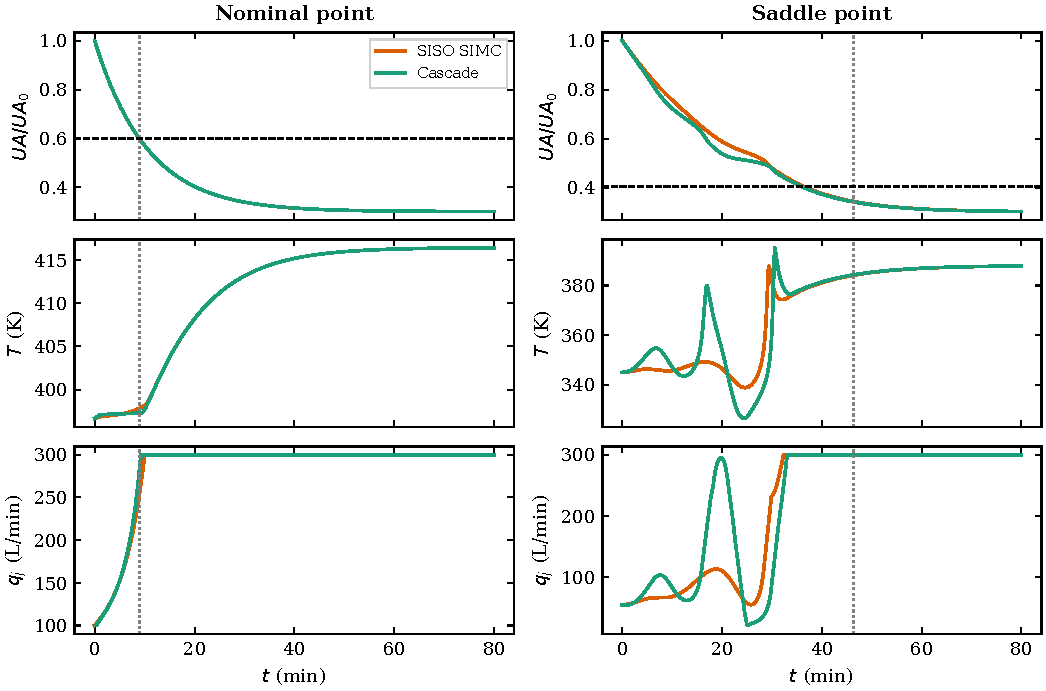
\includegraphics[width=\textwidth]{figures/fig4_fouling_runaway.pdf}
\caption{Continuous fouling at the nominal point (left) and at the saddle (right): heat-transfer capacity, reactor temperature and coolant flow. Dashed line: $UA_{\mathrm{crit}}$ from Eq.~\eqref{eq:ua_crit}; dotted line: $t_{\mathrm{pred}}$ from Eq.~\eqref{eq:t_pred}.}
\label{fig:fouling}
\end{figure*}

\paragraph{Nominal point: the thermodynamic limit is the binding one.} Both controllers hold the temperature while the valve opens, and the valve reaches $u_{\max}$ at $t_{\mathrm{sat}}=\tsatNomCascade$~min (cascade) and $\tsatNomSiso$~min (single loop), against $t_{\mathrm{pred}}=\tpredNom$~min from Eq.~\eqref{eq:t_pred}. The heat-transfer capacity at saturation, $\uaSatNomCascade\%$ and $\uaSatNomSiso\%$ of $UA_0$, is just below the $\fcritNom\%$ of Eq.~\eqref{eq:ua_crit}; the small delay is the tracking lag of each loop, larger for the slower single loop. After saturation the temperature leaves the setpoint ($t_{\mathrm{runaway}}=\trunNomCascade$~min for both) and climbs smoothly to $\TendNomCascade$~K, the stable equilibrium of the fouled reactor with the valve fully open. Because the nominal heat balance has a single root, there is no jump: the loss of regulation is a drift along the only branch, and its onset is predicted by a steady-state calculation.

\paragraph{Saddle: the loops fail long before the cooling capacity does.} At the saddle the quasi-steady prediction is $t_{\mathrm{pred}}=\tpredSad$~min, but neither loop gets there. The cascade first exceeds the $\bandRun$~K band at $\trunSadCascade$~min and the single loop at $\trunSadSiso$~min; both develop growing oscillations, the valve saturates during an excursion ($t_{\mathrm{sat}}=\tsatSadCascade$ and $\tsatSadSiso$~min), and the reactor ignites to the hot branch, ending at $\TendSadCascade$~K. The capacity at the moment of saturation, $\uaSatSadCascade\%$ and $\uaSatSadSiso\%$, is still above the critical $\fcritSad\%$: the valve did not saturate because the reactor needed more cooling than it could deliver, but because the loop had already become oscillatory.

\begin{figure}[t]
\centering
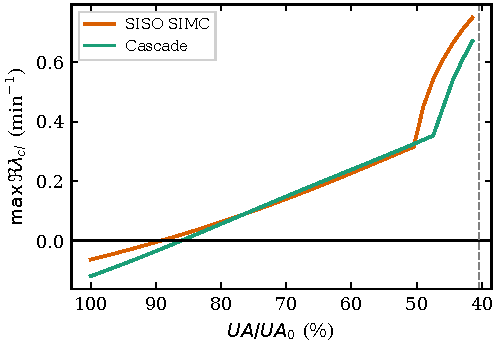
\includegraphics[width=\columnwidth]{figures/fig5_frozen_ua_stability.pdf}
\caption{Spectral abscissa of the linearized closed loop at the saddle for frozen values of $UA$, with gains tuned at $UA_0$. Dashed line: $UA_{\mathrm{crit}}$. Fixed-gain loops become unstable where the curves cross zero.}
\label{fig:frozen}
\end{figure}

Figure~\ref{fig:frozen} explains the mechanism. With gains fixed at their clean-jacket values, the linearized loops become unstable at $UA=\fstabSiso\%$ (single loop) and $\fstabCascade\%$ (cascade) of $UA_0$, where the equilibrium flows are only $\qstabSiso$ and $\qstabCascade$~L/min, far from the $\umax$~L/min of the valve. Fouling lowers the jacket temperature needed to hold the setpoint, which shrinks the actuator gain $b_3$ by a factor $\bThreeRatio$ between $UA_0$ and $UA_{\mathrm{crit}}$. For a controller that must keep $K_ck>1$ to hold an unstable pole (Section~\ref{subsec:siso_design}), losing actuator gain is losing stability. The cascade does not escape this: its slave loop acts on the same channel $b_3$, and once the slave is too weak the jacket coupling that it was cutting returns. In the fouling runs the cascade leaves the band earlier than the single loop most likely because the fast decline of $UA$ at the chosen $\kappa_{\mathrm{foul}}$ excites its less damped closed loop; the frozen-fouling boundary of Fig.~\ref{fig:frozen}, which does not depend on $\kappa_{\mathrm{foul}}$, shows that the two architectures lose the saddle at similar capacities.

The practical reading is that, on an open-loop unstable operating point, the controllability margin against fouling is not $UA_0-UA_{\mathrm{crit}}$ but $UA_0-UA_{\mathrm{stab}}$, and that the second is set by the controller rather than by the heat exchanger. Recovering the thermodynamic margin requires adapting the gain to the actuator effectiveness, for example by scheduling the slave gain on $1/(\bar T_j-T_{jf})$, which follows directly from Eq.~\eqref{eq:jacobian}; this is not tested here.

\subsection{Limitations}
The results rest on one reactor model with lumped, constant physical properties and perfect mixing. The saddle exists only with a feed cooled to $\TfSad$~K, a modification of the benchmark that we introduced because the nominal configuration has no unstable steady state; conclusions about the saddle should not be transferred to the nominal configuration, and the reverse. The fouling law of Eq.~\eqref{eq:fouling} is phenomenological and its rate constant is a scenario parameter chosen to keep the simulations short; only ratios to Eq.~\eqref{eq:t_pred} and the frozen-fouling boundaries are independent of it. Measurements are noise free, the valve has no stiction, and the controllers are PI only; derivative action, gain scheduling and model predictive control were not evaluated on the saddle \cite{rawlings2020model,andrade2026when}. The stability statements are local, based on the Jacobian, and are confirmed but not proven globally by the nonlinear simulations.
